\documentclass{article}
\usepackage[margin=1in]{geometry}
\usepackage{pgfplots}
\pgfplotsset{compat=1.18}
\pagestyle{empty}
\begin{document}
\begin{center}
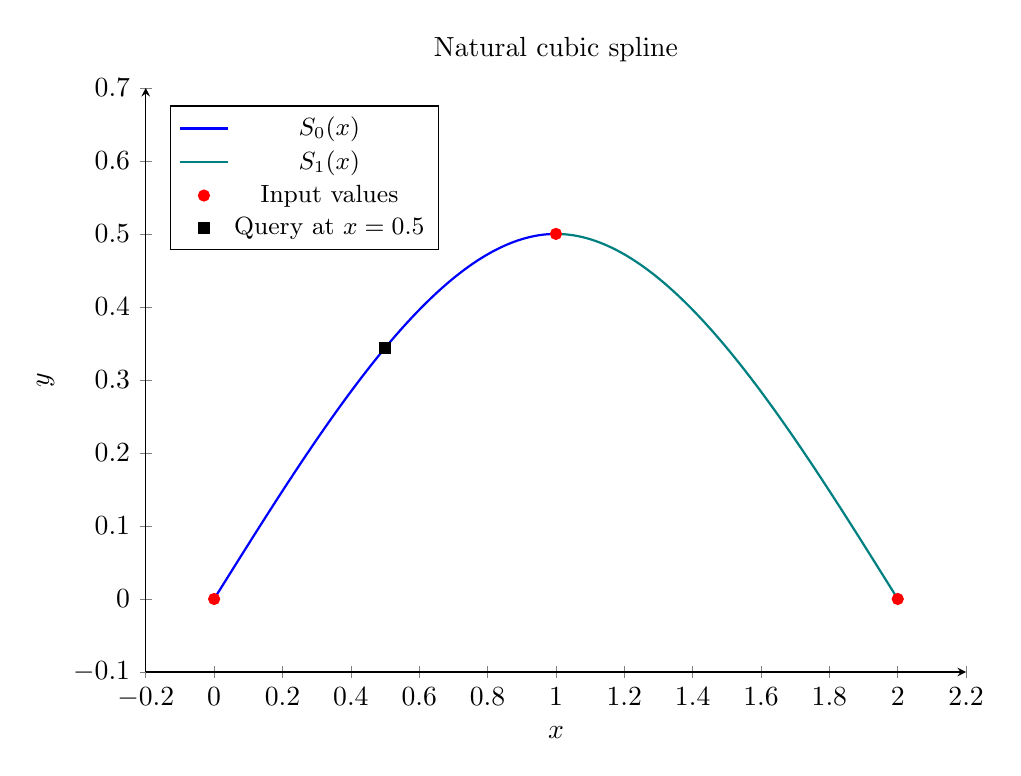
\begin{tikzpicture}
\begin{axis}[width=12cm,height=9cm,
axis lines=left,xlabel={$x$},ylabel={$y$},
legend pos=north west,legend style={font=\small},
xmin=-0.2,xmax=2.2,ymin=-0.1,ymax=0.7,
title={Natural cubic spline}]
\addplot[blue,thick,domain=0:1,samples=80] {0.75*x-0.25*x^3};
\addlegendentry{$S_0(x)$}
\addplot[teal,thick,domain=1:2,samples=80] {0.5-0.75*(x-1)^2+0.25*(x-1)^3};
\addlegendentry{$S_1(x)$}
\addplot[only marks,red] coordinates {(0,0) (1,0.5) (2,0)};
\addlegendentry{Input values}
\addplot[only marks,black,mark=square*] coordinates {(0.5,0.34375)};
\addlegendentry{Query at $x=0.5$}
\end{axis}
\end{tikzpicture}
\end{center}
\end{document}
